% Created by tikzDevice version 0.12.6 on 2024-11-19 16:55:34
% !TEX encoding = UTF-8 Unicode
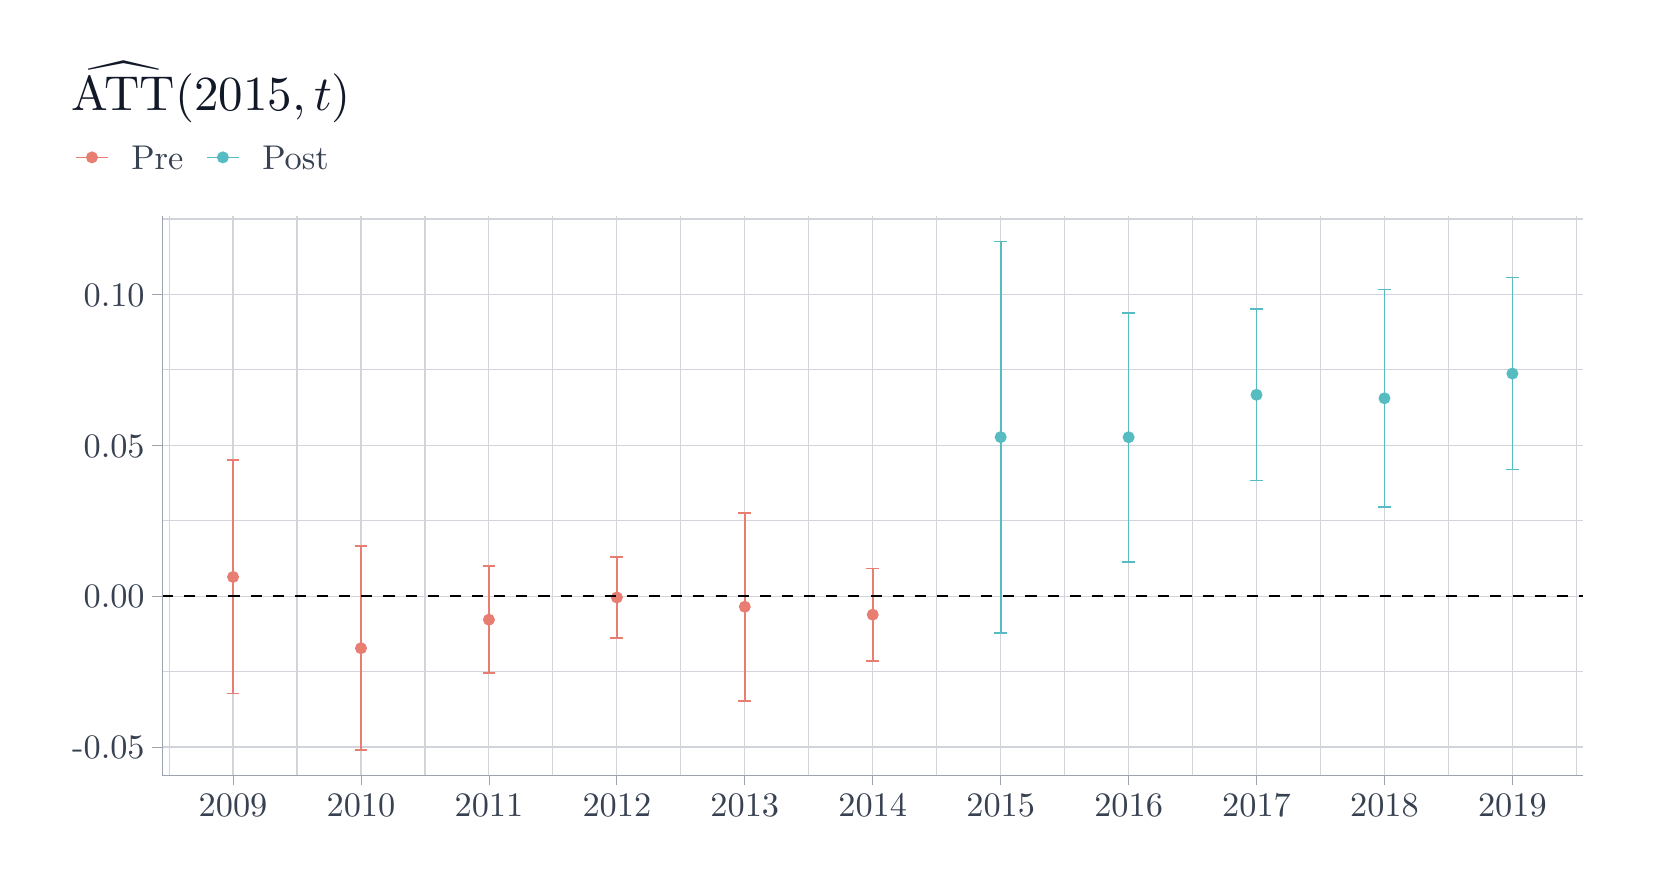
\begin{tikzpicture}[x=1pt,y=1pt]
\definecolor{fillColor}{RGB}{255,255,255}
\path[use as bounding box,fill=fillColor] (0,0) rectangle (578.16,303.53);
\begin{scope}
\path[clip] (  0.00,  0.00) rectangle (578.16,303.53);
\definecolor{drawColor}{RGB}{255,255,255}

\path[draw=drawColor,line width= 0.7pt,line join=round,line cap=round,fill=fillColor] (  0.00,  0.00) rectangle (578.16,303.53);
\end{scope}
\begin{scope}
\path[clip] ( 48.56, 33.29) rectangle (562.16,235.43);
\definecolor{drawColor}{RGB}{255,255,255}
\definecolor{fillColor}{RGB}{255,255,255}

\path[draw=drawColor,line width= 0.7pt,line join=round,line cap=round,fill=fillColor] ( 48.56, 33.29) rectangle (562.16,235.43);
\definecolor{drawColor}{RGB}{209,213,219}

\path[draw=drawColor,line width= 0.4pt,line join=round] ( 48.56, 70.87) --
	(562.16, 70.87);

\path[draw=drawColor,line width= 0.4pt,line join=round] ( 48.56,125.38) --
	(562.16,125.38);

\path[draw=drawColor,line width= 0.4pt,line join=round] ( 48.56,179.88) --
	(562.16,179.88);

\path[draw=drawColor,line width= 0.4pt,line join=round] ( 48.56,234.39) --
	(562.16,234.39);

\path[draw=drawColor,line width= 0.4pt,line join=round] ( 51.10, 33.29) --
	( 51.10,235.43);

\path[draw=drawColor,line width= 0.4pt,line join=round] ( 97.33, 33.29) --
	( 97.33,235.43);

\path[draw=drawColor,line width= 0.4pt,line join=round] (143.56, 33.29) --
	(143.56,235.43);

\path[draw=drawColor,line width= 0.4pt,line join=round] (189.79, 33.29) --
	(189.79,235.43);

\path[draw=drawColor,line width= 0.4pt,line join=round] (236.01, 33.29) --
	(236.01,235.43);

\path[draw=drawColor,line width= 0.4pt,line join=round] (282.24, 33.29) --
	(282.24,235.43);

\path[draw=drawColor,line width= 0.4pt,line join=round] (328.47, 33.29) --
	(328.47,235.43);

\path[draw=drawColor,line width= 0.4pt,line join=round] (374.70, 33.29) --
	(374.70,235.43);

\path[draw=drawColor,line width= 0.4pt,line join=round] (420.93, 33.29) --
	(420.93,235.43);

\path[draw=drawColor,line width= 0.4pt,line join=round] (467.16, 33.29) --
	(467.16,235.43);

\path[draw=drawColor,line width= 0.4pt,line join=round] (513.39, 33.29) --
	(513.39,235.43);

\path[draw=drawColor,line width= 0.4pt,line join=round] (559.62, 33.29) --
	(559.62,235.43);

\path[draw=drawColor,line width= 0.4pt,line join=round] ( 48.56, 43.61) --
	(562.16, 43.61);

\path[draw=drawColor,line width= 0.4pt,line join=round] ( 48.56, 98.12) --
	(562.16, 98.12);

\path[draw=drawColor,line width= 0.4pt,line join=round] ( 48.56,152.63) --
	(562.16,152.63);

\path[draw=drawColor,line width= 0.4pt,line join=round] ( 48.56,207.14) --
	(562.16,207.14);

\path[draw=drawColor,line width= 0.4pt,line join=round] ( 74.21, 33.29) --
	( 74.21,235.43);

\path[draw=drawColor,line width= 0.4pt,line join=round] (120.44, 33.29) --
	(120.44,235.43);

\path[draw=drawColor,line width= 0.4pt,line join=round] (166.67, 33.29) --
	(166.67,235.43);

\path[draw=drawColor,line width= 0.4pt,line join=round] (212.90, 33.29) --
	(212.90,235.43);

\path[draw=drawColor,line width= 0.4pt,line join=round] (259.13, 33.29) --
	(259.13,235.43);

\path[draw=drawColor,line width= 0.4pt,line join=round] (305.36, 33.29) --
	(305.36,235.43);

\path[draw=drawColor,line width= 0.4pt,line join=round] (351.59, 33.29) --
	(351.59,235.43);

\path[draw=drawColor,line width= 0.4pt,line join=round] (397.82, 33.29) --
	(397.82,235.43);

\path[draw=drawColor,line width= 0.4pt,line join=round] (444.04, 33.29) --
	(444.04,235.43);

\path[draw=drawColor,line width= 0.4pt,line join=round] (490.27, 33.29) --
	(490.27,235.43);

\path[draw=drawColor,line width= 0.4pt,line join=round] (536.50, 33.29) --
	(536.50,235.43);
\definecolor{drawColor}{RGB}{232,125,114}
\definecolor{fillColor}{RGB}{232,125,114}

\path[draw=drawColor,line width= 0.4pt,line join=round,line cap=round,fill=fillColor] ( 74.21,105.04) circle (  1.96);

\path[draw=drawColor,line width= 0.4pt,line join=round,line cap=round,fill=fillColor] (120.44, 79.30) circle (  1.96);

\path[draw=drawColor,line width= 0.4pt,line join=round,line cap=round,fill=fillColor] (166.67, 89.61) circle (  1.96);

\path[draw=drawColor,line width= 0.4pt,line join=round,line cap=round,fill=fillColor] (212.90, 97.63) circle (  1.96);

\path[draw=drawColor,line width= 0.4pt,line join=round,line cap=round,fill=fillColor] (259.13, 94.28) circle (  1.96);

\path[draw=drawColor,line width= 0.4pt,line join=round,line cap=round,fill=fillColor] (305.36, 91.42) circle (  1.96);
\definecolor{drawColor}{RGB}{86,188,194}
\definecolor{fillColor}{RGB}{86,188,194}

\path[draw=drawColor,line width= 0.4pt,line join=round,line cap=round,fill=fillColor] (351.59,155.57) circle (  1.96);

\path[draw=drawColor,line width= 0.4pt,line join=round,line cap=round,fill=fillColor] (397.82,155.53) circle (  1.96);

\path[draw=drawColor,line width= 0.4pt,line join=round,line cap=round,fill=fillColor] (444.04,170.87) circle (  1.96);

\path[draw=drawColor,line width= 0.4pt,line join=round,line cap=round,fill=fillColor] (490.27,169.61) circle (  1.96);

\path[draw=drawColor,line width= 0.4pt,line join=round,line cap=round,fill=fillColor] (536.50,178.54) circle (  1.96);
\definecolor{drawColor}{RGB}{232,125,114}

\path[draw=drawColor,line width= 0.6pt,line join=round] ( 71.90,147.20) --
	( 76.52,147.20);

\path[draw=drawColor,line width= 0.6pt,line join=round] ( 74.21,147.20) --
	( 74.21, 62.89);

\path[draw=drawColor,line width= 0.6pt,line join=round] ( 71.90, 62.89) --
	( 76.52, 62.89);

\path[draw=drawColor,line width= 0.6pt,line join=round] (118.13,116.12) --
	(122.75,116.12);

\path[draw=drawColor,line width= 0.6pt,line join=round] (120.44,116.12) --
	(120.44, 42.47);

\path[draw=drawColor,line width= 0.6pt,line join=round] (118.13, 42.47) --
	(122.75, 42.47);

\path[draw=drawColor,line width= 0.6pt,line join=round] (164.36,108.94) --
	(168.98,108.94);

\path[draw=drawColor,line width= 0.6pt,line join=round] (166.67,108.94) --
	(166.67, 70.27);

\path[draw=drawColor,line width= 0.6pt,line join=round] (164.36, 70.27) --
	(168.98, 70.27);

\path[draw=drawColor,line width= 0.6pt,line join=round] (210.59,112.35) --
	(215.21,112.35);

\path[draw=drawColor,line width= 0.6pt,line join=round] (212.90,112.35) --
	(212.90, 82.90);

\path[draw=drawColor,line width= 0.6pt,line join=round] (210.59, 82.90) --
	(215.21, 82.90);

\path[draw=drawColor,line width= 0.6pt,line join=round] (256.82,128.22) --
	(261.44,128.22);

\path[draw=drawColor,line width= 0.6pt,line join=round] (259.13,128.22) --
	(259.13, 60.34);

\path[draw=drawColor,line width= 0.6pt,line join=round] (256.82, 60.34) --
	(261.44, 60.34);

\path[draw=drawColor,line width= 0.6pt,line join=round] (303.05,108.12) --
	(307.67,108.12);

\path[draw=drawColor,line width= 0.6pt,line join=round] (305.36,108.12) --
	(305.36, 74.72);

\path[draw=drawColor,line width= 0.6pt,line join=round] (303.05, 74.72) --
	(307.67, 74.72);
\definecolor{drawColor}{RGB}{86,188,194}

\path[draw=drawColor,line width= 0.6pt,line join=round] (349.28,226.24) --
	(353.90,226.24);

\path[draw=drawColor,line width= 0.6pt,line join=round] (351.59,226.24) --
	(351.59, 84.89);

\path[draw=drawColor,line width= 0.6pt,line join=round] (349.28, 84.89) --
	(353.90, 84.89);

\path[draw=drawColor,line width= 0.6pt,line join=round] (395.50,200.53) --
	(400.13,200.53);

\path[draw=drawColor,line width= 0.6pt,line join=round] (397.82,200.53) --
	(397.82,110.52);

\path[draw=drawColor,line width= 0.6pt,line join=round] (395.50,110.52) --
	(400.13,110.52);

\path[draw=drawColor,line width= 0.6pt,line join=round] (441.73,201.88) --
	(446.36,201.88);

\path[draw=drawColor,line width= 0.6pt,line join=round] (444.04,201.88) --
	(444.04,139.85);

\path[draw=drawColor,line width= 0.6pt,line join=round] (441.73,139.85) --
	(446.36,139.85);

\path[draw=drawColor,line width= 0.6pt,line join=round] (487.96,208.92) --
	(492.59,208.92);

\path[draw=drawColor,line width= 0.6pt,line join=round] (490.27,208.92) --
	(490.27,130.29);

\path[draw=drawColor,line width= 0.6pt,line join=round] (487.96,130.29) --
	(492.59,130.29);

\path[draw=drawColor,line width= 0.6pt,line join=round] (534.19,213.26) --
	(538.81,213.26);

\path[draw=drawColor,line width= 0.6pt,line join=round] (536.50,213.26) --
	(536.50,143.83);

\path[draw=drawColor,line width= 0.6pt,line join=round] (534.19,143.83) --
	(538.81,143.83);
\definecolor{drawColor}{RGB}{0,0,0}

\path[draw=drawColor,line width= 0.6pt,dash pattern=on 4pt off 4pt ,line join=round] ( 48.56, 98.12) -- (562.16, 98.12);
\end{scope}
\begin{scope}
\path[clip] (  0.00,  0.00) rectangle (578.16,303.53);
\definecolor{drawColor}{RGB}{156,163,175}

\path[draw=drawColor,line width= 0.3pt,line join=round] ( 48.56, 33.29) --
	( 48.56,235.43);
\end{scope}
\begin{scope}
\path[clip] (  0.00,  0.00) rectangle (578.16,303.53);
\definecolor{drawColor}{RGB}{55,65,81}

\node[text=drawColor,anchor=base east,inner sep=0pt, outer sep=0pt, scale=  1.24] at ( 42.26, 39.33) {-0.05};

\node[text=drawColor,anchor=base east,inner sep=0pt, outer sep=0pt, scale=  1.24] at ( 42.26, 93.84) {0.00};

\node[text=drawColor,anchor=base east,inner sep=0pt, outer sep=0pt, scale=  1.24] at ( 42.26,148.35) {0.05};

\node[text=drawColor,anchor=base east,inner sep=0pt, outer sep=0pt, scale=  1.24] at ( 42.26,202.85) {0.10};
\end{scope}
\begin{scope}
\path[clip] (  0.00,  0.00) rectangle (578.16,303.53);
\definecolor{drawColor}{RGB}{156,163,175}

\path[draw=drawColor,line width= 0.3pt,line join=round] ( 45.06, 43.61) --
	( 48.56, 43.61);

\path[draw=drawColor,line width= 0.3pt,line join=round] ( 45.06, 98.12) --
	( 48.56, 98.12);

\path[draw=drawColor,line width= 0.3pt,line join=round] ( 45.06,152.63) --
	( 48.56,152.63);

\path[draw=drawColor,line width= 0.3pt,line join=round] ( 45.06,207.14) --
	( 48.56,207.14);
\end{scope}
\begin{scope}
\path[clip] (  0.00,  0.00) rectangle (578.16,303.53);
\definecolor{drawColor}{RGB}{156,163,175}

\path[draw=drawColor,line width= 0.3pt,line join=round] ( 48.56, 33.29) --
	(562.16, 33.29);
\end{scope}
\begin{scope}
\path[clip] (  0.00,  0.00) rectangle (578.16,303.53);
\definecolor{drawColor}{RGB}{156,163,175}

\path[draw=drawColor,line width= 0.3pt,line join=round] ( 74.21, 29.79) --
	( 74.21, 33.29);

\path[draw=drawColor,line width= 0.3pt,line join=round] (120.44, 29.79) --
	(120.44, 33.29);

\path[draw=drawColor,line width= 0.3pt,line join=round] (166.67, 29.79) --
	(166.67, 33.29);

\path[draw=drawColor,line width= 0.3pt,line join=round] (212.90, 29.79) --
	(212.90, 33.29);

\path[draw=drawColor,line width= 0.3pt,line join=round] (259.13, 29.79) --
	(259.13, 33.29);

\path[draw=drawColor,line width= 0.3pt,line join=round] (305.36, 29.79) --
	(305.36, 33.29);

\path[draw=drawColor,line width= 0.3pt,line join=round] (351.59, 29.79) --
	(351.59, 33.29);

\path[draw=drawColor,line width= 0.3pt,line join=round] (397.82, 29.79) --
	(397.82, 33.29);

\path[draw=drawColor,line width= 0.3pt,line join=round] (444.04, 29.79) --
	(444.04, 33.29);

\path[draw=drawColor,line width= 0.3pt,line join=round] (490.27, 29.79) --
	(490.27, 33.29);

\path[draw=drawColor,line width= 0.3pt,line join=round] (536.50, 29.79) --
	(536.50, 33.29);
\end{scope}
\begin{scope}
\path[clip] (  0.00,  0.00) rectangle (578.16,303.53);
\definecolor{drawColor}{RGB}{55,65,81}

\node[text=drawColor,anchor=base,inner sep=0pt, outer sep=0pt, scale=  1.24] at ( 74.21, 18.42) {2009};

\node[text=drawColor,anchor=base,inner sep=0pt, outer sep=0pt, scale=  1.24] at (120.44, 18.42) {2010};

\node[text=drawColor,anchor=base,inner sep=0pt, outer sep=0pt, scale=  1.24] at (166.67, 18.42) {2011};

\node[text=drawColor,anchor=base,inner sep=0pt, outer sep=0pt, scale=  1.24] at (212.90, 18.42) {2012};

\node[text=drawColor,anchor=base,inner sep=0pt, outer sep=0pt, scale=  1.24] at (259.13, 18.42) {2013};

\node[text=drawColor,anchor=base,inner sep=0pt, outer sep=0pt, scale=  1.24] at (305.36, 18.42) {2014};

\node[text=drawColor,anchor=base,inner sep=0pt, outer sep=0pt, scale=  1.24] at (351.59, 18.42) {2015};

\node[text=drawColor,anchor=base,inner sep=0pt, outer sep=0pt, scale=  1.24] at (397.82, 18.42) {2016};

\node[text=drawColor,anchor=base,inner sep=0pt, outer sep=0pt, scale=  1.24] at (444.04, 18.42) {2017};

\node[text=drawColor,anchor=base,inner sep=0pt, outer sep=0pt, scale=  1.24] at (490.27, 18.42) {2018};

\node[text=drawColor,anchor=base,inner sep=0pt, outer sep=0pt, scale=  1.24] at (536.50, 18.42) {2019};
\end{scope}
\begin{scope}
\path[clip] (  0.00,  0.00) rectangle (578.16,303.53);
\definecolor{drawColor}{RGB}{255,255,255}
\definecolor{fillColor}{RGB}{255,255,255}

\path[draw=drawColor,line width= 0.7pt,line join=round,line cap=round,fill=fillColor] ( 16.00,249.43) rectangle (108.85,263.89);
\end{scope}
\begin{scope}
\path[clip] (  0.00,  0.00) rectangle (578.16,303.53);
\definecolor{drawColor}{RGB}{255,255,255}
\definecolor{fillColor}{RGB}{255,255,255}

\path[draw=drawColor,line width= 0.7pt,line join=round,line cap=round,fill=fillColor] ( 16.00,249.43) rectangle ( 30.45,263.89);
\end{scope}
\begin{scope}
\path[clip] (  0.00,  0.00) rectangle (578.16,303.53);
\definecolor{drawColor}{RGB}{232,125,114}
\definecolor{fillColor}{RGB}{232,125,114}

\path[draw=drawColor,line width= 0.4pt,line join=round,line cap=round,fill=fillColor] ( 23.23,256.66) circle (  1.96);
\end{scope}
\begin{scope}
\path[clip] (  0.00,  0.00) rectangle (578.16,303.53);
\definecolor{drawColor}{RGB}{232,125,114}

\path[draw=drawColor,line width= 0.6pt,line join=round] ( 17.45,256.66) -- ( 29.01,256.66);
\end{scope}
\begin{scope}
\path[clip] (  0.00,  0.00) rectangle (578.16,303.53);
\definecolor{drawColor}{RGB}{255,255,255}
\definecolor{fillColor}{RGB}{255,255,255}

\path[draw=drawColor,line width= 0.7pt,line join=round,line cap=round,fill=fillColor] ( 63.32,249.43) rectangle ( 77.77,263.89);
\end{scope}
\begin{scope}
\path[clip] (  0.00,  0.00) rectangle (578.16,303.53);
\definecolor{drawColor}{RGB}{86,188,194}
\definecolor{fillColor}{RGB}{86,188,194}

\path[draw=drawColor,line width= 0.4pt,line join=round,line cap=round,fill=fillColor] ( 70.54,256.66) circle (  1.96);
\end{scope}
\begin{scope}
\path[clip] (  0.00,  0.00) rectangle (578.16,303.53);
\definecolor{drawColor}{RGB}{86,188,194}

\path[draw=drawColor,line width= 0.6pt,line join=round] ( 64.76,256.66) -- ( 76.33,256.66);
\end{scope}
\begin{scope}
\path[clip] (  0.00,  0.00) rectangle (578.16,303.53);
\definecolor{drawColor}{RGB}{55,65,81}

\node[text=drawColor,anchor=base west,inner sep=0pt, outer sep=0pt, scale=  1.24] at ( 37.45,252.37) {Pre};
\end{scope}
\begin{scope}
\path[clip] (  0.00,  0.00) rectangle (578.16,303.53);
\definecolor{drawColor}{RGB}{55,65,81}

\node[text=drawColor,anchor=base west,inner sep=0pt, outer sep=0pt, scale=  1.24] at ( 84.77,252.37) {Post};
\end{scope}
\begin{scope}
\path[clip] (  0.00,  0.00) rectangle (578.16,303.53);
\definecolor{drawColor}{RGB}{17,24,39}

\node[text=drawColor,anchor=base west,inner sep=0pt, outer sep=0pt, scale=  1.77] at ( 16.00,273.61) {$\widehat{\textrm{ATT}}(2015, t)$};
\end{scope}
\end{tikzpicture}
